\documentclass{beamer} %
\usetheme{CambridgeUS}
\usepackage[latin1]{inputenc}
\usefonttheme{professionalfonts}
\usepackage{times}
\usepackage{tikz}
\usepackage{amsmath}
\usepackage{verbatim}
\usetikzlibrary{arrows,shapes}
\usepackage[ruled,vlined]{algorithm2e}

\usepackage{listings}
\usepackage{xcolor}
\lstset{
    language=Python,
    basicstyle=\ttfamily\small,
    keywordstyle=\color{blue},
    commentstyle=\color{gray},
    stringstyle=\color{red},
    showstringspaces=false,
    breaklines=true,
    frame=single
}

\title{Comparing Model Architectures with k-Fold Cross-Validation}
\author{Fernando Pujaico Rivera}
\date{}

\begin{document}

\frame{\titlepage}

%------------------------------------------------

\begin{frame}{A performs better than B?}
\begin{figure}
 \centering
 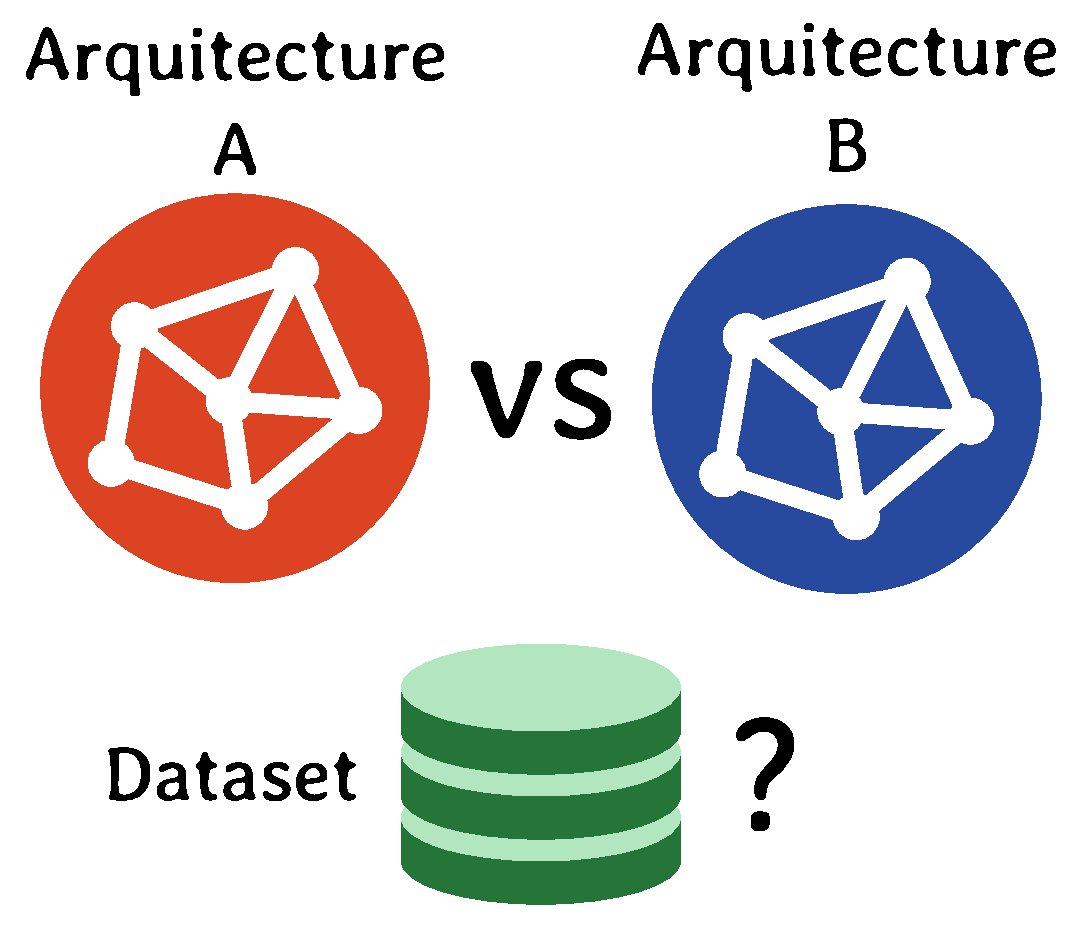
\includegraphics[width=0.65\linewidth]{dilema.pdf}
 % dilema.pdf: 519x445 px, 72dpi, 18.31x15.70 cm, bb=0 0 519 445
\end{figure}
\end{frame}

%------------------------------------------------

\begin{frame}{Problem}

\begin{description}
\item[Goal:] determine whether \textbf{Architecture A performs better than Architecture B}.
\bigskip
\item[Method:] \textbf{k-fold cross-validation} + \textbf{t-test}
\bigskip
\item[Objective:]
\begin{itemize}
\item Obtain multiple performance estimates
\item Perform a \textbf{statistical comparison between architectures}
\end{itemize}
\end{description}

\end{frame}

%------------------------------------------------

\begin{frame}{k-Fold Cross-Validation}

\includegraphics[width=0.03\linewidth]{dataset.pdf}
Dataset is divided into $K$ folds. If $K=5$, then

\begin{figure}
 \centering
 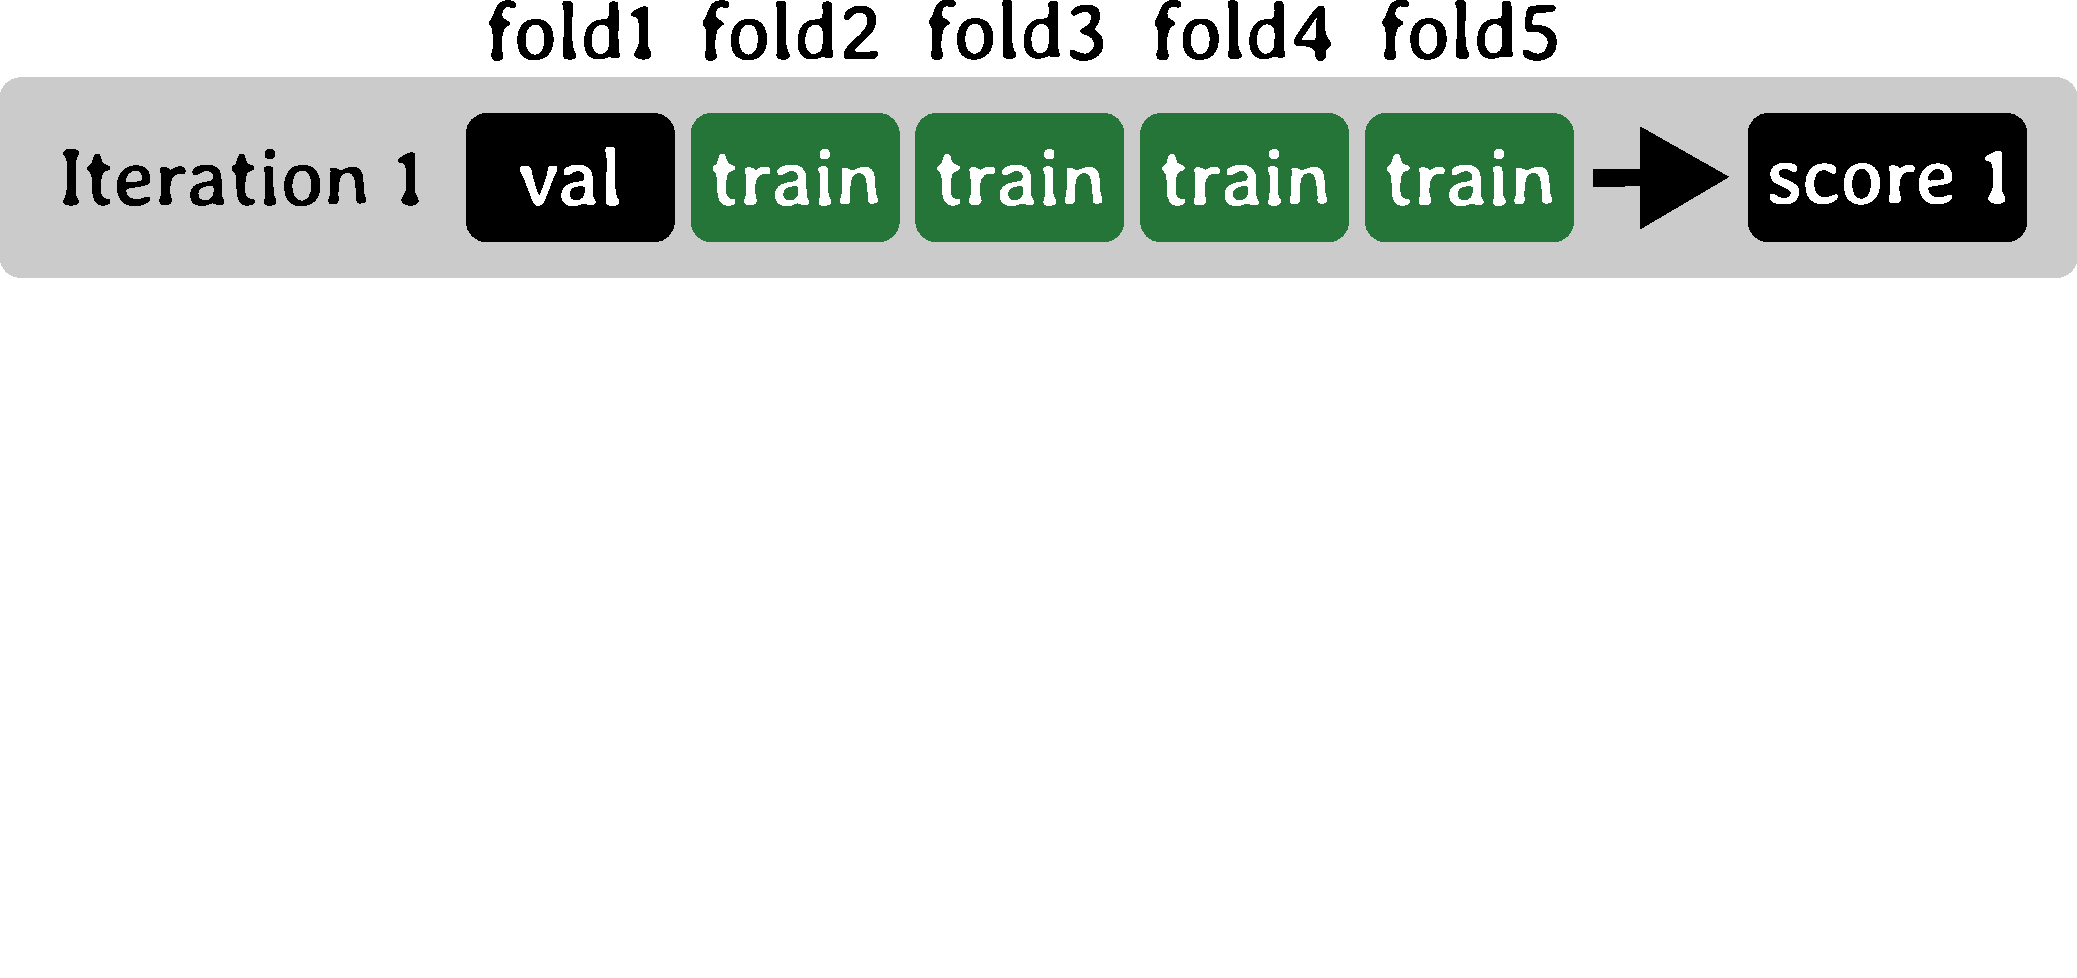
\includegraphics[width=0.95\linewidth]{kfold0.pdf}
 \end{figure}

\end{frame}

\begin{frame}{k-Fold Cross-Validation}

\includegraphics[width=0.03\linewidth]{dataset.pdf}
Dataset is divided into $K$ folds. If $K=5$, then

\begin{figure}
 \centering
 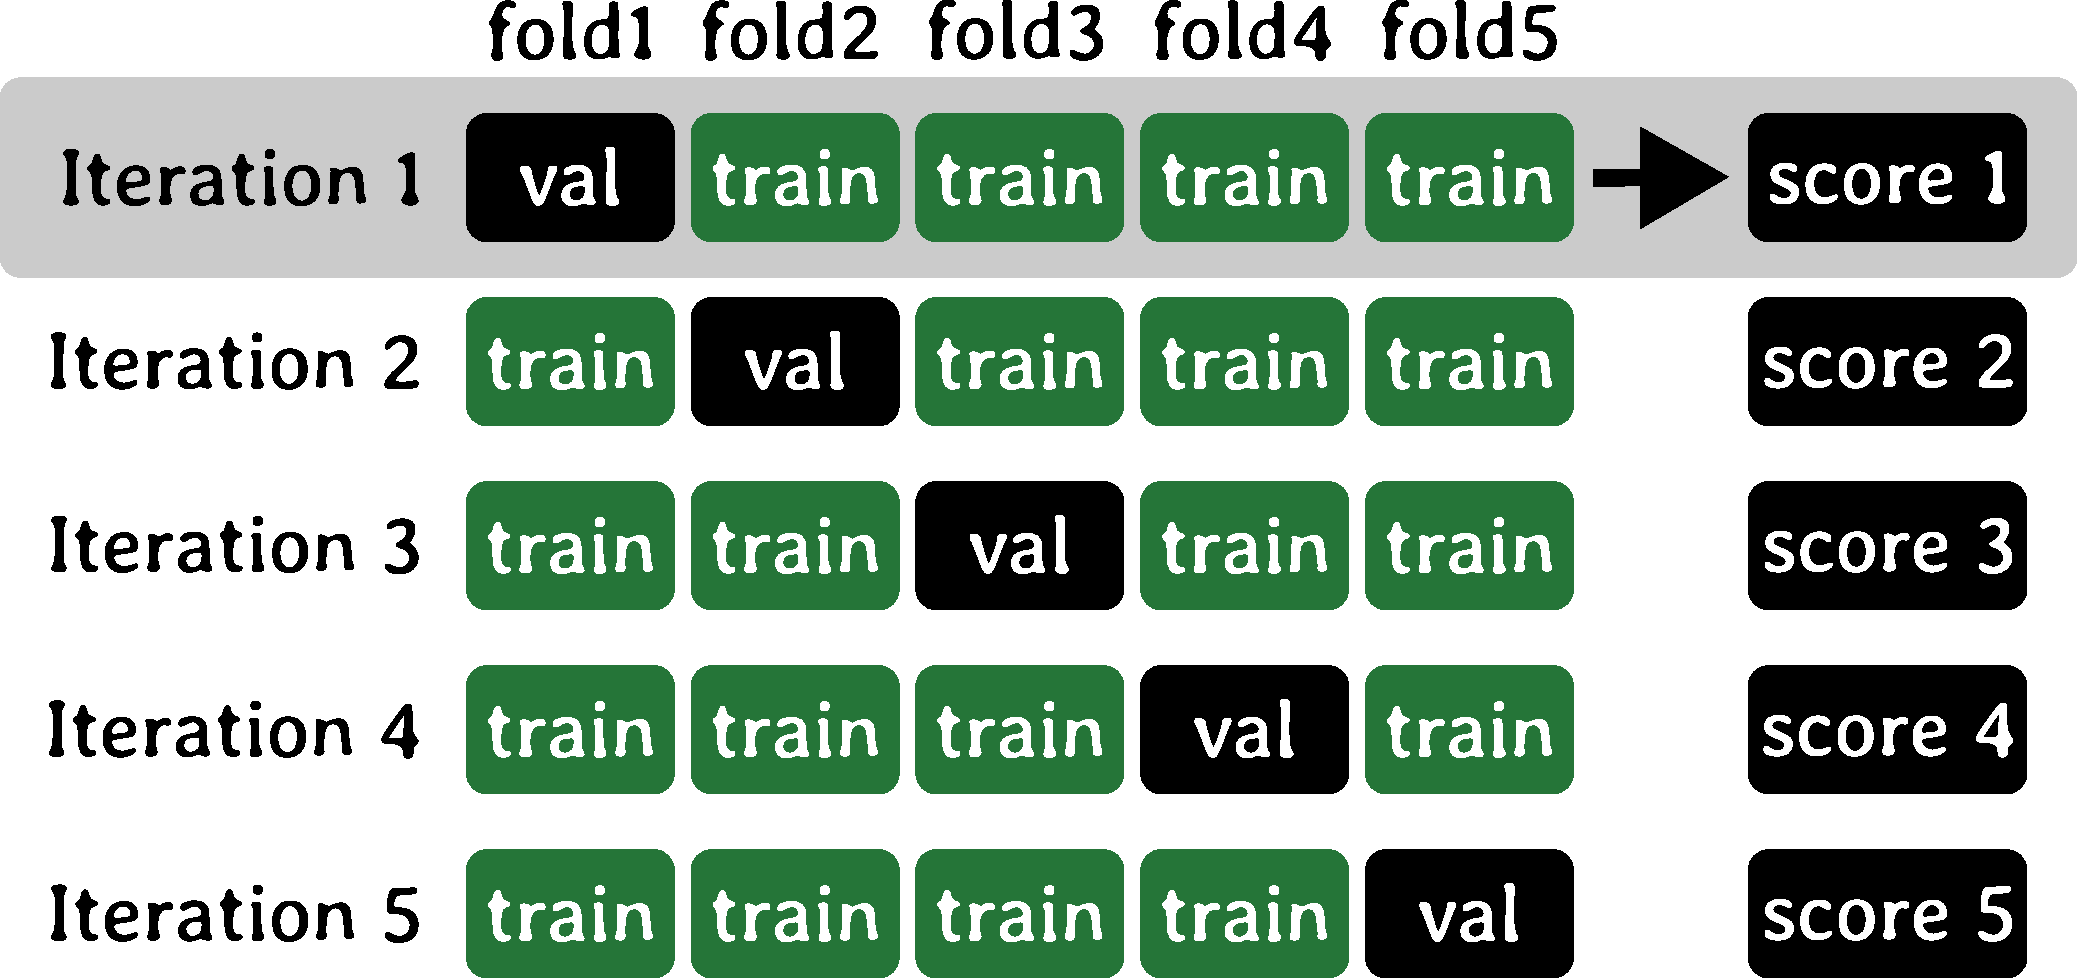
\includegraphics[width=0.95\linewidth]{kfold.pdf}
 \end{figure}

\end{frame}
%------------------------------------------------

\begin{frame}{K-Fold Cross-Validation}
Example with $K = 5$.



\begin{center}
\begin{tabular}{c|c|c}
     & 
\includegraphics[width=0.05\linewidth]{arq-a.pdf} & 
\includegraphics[width=0.05\linewidth]{arq-b.pdf} \\
Validation fold & Score A & Score B \\
\hline
1 & $a_1$ & $b_1$ \\
2 & $a_2$ & $b_2$ \\
3 & $a_3$ & $b_3$ \\
4 & $a_4$ & $b_4$ \\
5 & $a_5$ & $b_5$
\end{tabular}
\end{center}

\[
\mu_A =\frac{1}{K}\sum\limits_{k=1}^{K} a_{k}
\qquad\wedge\qquad
\mu_B =\frac{1}{K}\sum\limits_{k=1}^{K} b_{k}
\]

\bigskip

\end{frame}

%------------------------------------------------

\begin{frame}{Comparison}
\begin{figure}
 \centering
 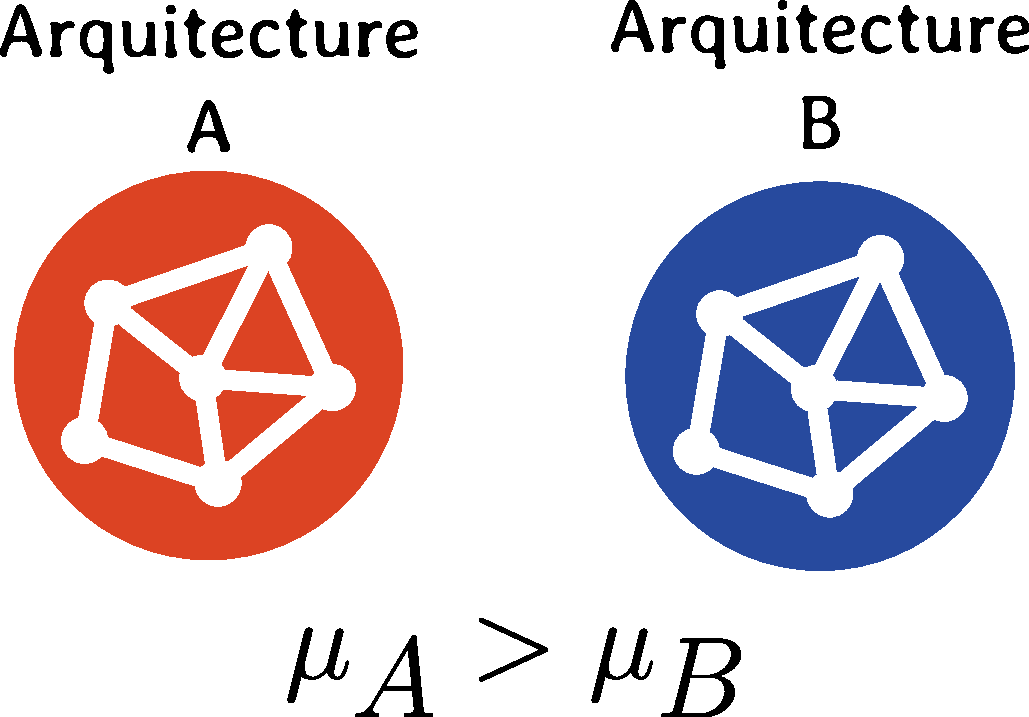
\includegraphics[width=0.65\linewidth]{problem.pdf}
\end{figure}
\end{frame}

%------------------------------------------------

\begin{frame}{Comparison method}
\begin{center}
\Huge
\textcolor{blue}{One-sided} \textcolor{red}{paired} t-test
\end{center}
\bigskip
{\Large
\textbf{Requirements:}{ Normality condition of analyzed data}
}
\end{frame}

%------------------------------------------------

\begin{frame}{Paired Comparison}

Because both models use the \textbf{same folds}, the comparison is \textbf{paired}.

For each fold we compute the difference: $d_k = a_k - b_k$

\bigskip

\begin{center}
\begin{tabular}{c|c|c|c}
Validation fold & Score A & Score B & $d_k$ \\
\hline
1 & 0.82 & 0.80 & 0.02 \\
2 & 0.79 & 0.76 & 0.03 \\
3 & 0.83 & 0.81 & 0.02 \\
4 & 0.81 & 0.78 & 0.03 \\
5 & 0.80 & 0.78 & 0.02
\end{tabular}
\end{center}

\bigskip

Statistical analysis is performed on the \textbf{vector of differences}:
\[
d = [d_1, d_2, d_3, d_4, d_5]
\]

\end{frame}

%------------------------------------------------

\begin{frame}[fragile]{Normality Test (Shapiro-Wilk)}
The one-sided paired t-test assumes that the differences follow a normal distribution.
We test the normality of the differences vector:
\[
d = [d_1, d_2, d_3, d_4, d_5]
\]

\begin{lstlisting}
import numpy as np
from scipy import stats

ScoreA = np.array([0.82, 0.79, 0.83, 0.81, 0.80])
ScoreB = np.array([0.80, 0.76, 0.81, 0.78, 0.78])
d = ScoreA - ScoreB

w, p = stats.shapiro(d)
if p > 0.05: # W close to 1.0 indicate normality.
    print("Differences are normally distributed")
\end{lstlisting}
\end{frame}

%------------------------------------------------

\begin{frame}{One sided paired t-test}

We test whether the \textbf{mean difference} is greater than zero.
\bigskip
\begin{description}
\item[Null hypothesis:]

\[
H_0 : \mu_A \le \mu_B
\]

\item[Alternative hypothesis:]
\[
H_1 : \mu_A > \mu_B
\]
\end{description}

\bigskip
Apply a \textcolor{red}{one-sided paired t-test} to test whether $\mu_A > \mu_B$.

\bigskip

Decision rule:

\begin{center}
\textbf{$p < 0.05$ $\Rightarrow$ significant difference}
\end{center}

\end{frame}

%------------------------------------------------

\begin{frame}[fragile]{One-sided paired t-test in Python}

If the differences are normally distributed, we apply a one-sided paired t-test.

\bigskip

Python example:

\begin{lstlisting}
import numpy as np
from scipy import stats

A = np.array([0.82, 0.79, 0.83, 0.81, 0.80])
B = np.array([0.80, 0.76, 0.81, 0.78, 0.78])

t, p = stats.ttest_rel(A, B, alternative="greater")

if p < 0.05:
    print("A performs significantly better than B")
\end{lstlisting}

\end{frame}

%------------------------------------------------

\begin{frame}{Conclusion}

Procedure:

\begin{enumerate}
\item Train models using \textbf{k-fold cross-validation}
\item Obtain \textbf{k scores per architecture}
\item Check normality distribution of \textbf{fold-wise score differences}
\item Apply a \textbf{one-sided paired t-test} to get the $p$ value
\end{enumerate}

\bigskip

\begin{algorithm}[H]
\eIf{$p < 0.05$}{
    Architecture $A$ performs better than Architecture $B$\;
}{
    No significant difference\;
}
\end{algorithm}

\end{frame}

\end{document}
